\documentclass[11pt,a4paper]{report}
\usepackage[textwidth=37em,vmargin=30mm]{geometry}
\usepackage{calc,xunicode,amsmath,amssymb,paralist,enumitem,tabu,booktabs,datetime2,xeCJK,xeCJKfntef,listings}
\usepackage{tocloft,fancyhdr,tcolorbox,xcolor,graphicx,eso-pic,xltxtra,xelatexemoji}

\newcommand{\envyear}[0]{2025}
\newcommand{\envdatestr}[0]{2025-02-10}
\newcommand{\envfinaldir}[0]{webdb/2025/20250210/final}

\usepackage[hidelinks]{hyperref}
\hypersetup{
    colorlinks=false,
    pdfpagemode=FullScreen,
    pdftitle={Web Digest - \envdatestr}
}

\setlength{\cftbeforechapskip}{10pt}
\renewcommand{\cftchapfont}{\rmfamily\bfseries\large\raggedright}
\setlength{\cftbeforesecskip}{2pt}
\renewcommand{\cftsecfont}{\sffamily\small\raggedright}

\setdefaultleftmargin{2em}{2em}{1em}{1em}{1em}{1em}

\usepackage{xeCJK,xeCJKfntef}
\xeCJKsetup{PunctStyle=plain,RubberPunctSkip=false,CJKglue=\strut\hskip 0pt plus 0.1em minus 0.05em,CJKecglue=\strut\hskip 0.22em plus 0.2em}
\XeTeXlinebreaklocale "zh"
\XeTeXlinebreakskip = 0pt


\setmainfont{Brygada 1918}
\setromanfont{Brygada 1918}
\setsansfont{IBM Plex Sans}
\setmonofont{JetBrains Mono NL}
\setCJKmainfont{Noto Serif CJK SC}
\setCJKromanfont{Noto Serif CJK SC}
\setCJKsansfont{Noto Sans CJK SC}
\setCJKmonofont{Noto Sans CJK SC}

\setlength{\parindent}{0pt}
\setlength{\parskip}{8pt}
\linespread{1.15}

\lstset{
	basicstyle=\ttfamily\footnotesize,
	numbersep=5pt,
	backgroundcolor=\color{black!5},
	showspaces=false,
	showstringspaces=false,
	showtabs=false,
	tabsize=2,
	captionpos=b,
	breaklines=true,
	breakatwhitespace=true,
	breakautoindent=true,
	linewidth=\textwidth
}






\newcommand{\coverpic}[2]{
    % argv: itemurl, authorname
    Cover photo by #2~~(\href{#1}{#1})
}
\newcommand{\makeheader}[0]{
    \begin{titlepage}
        % \newgeometry{hmargin=15mm,tmargin=21mm,bmargin=12mm}
        \begin{center}
            
            \rmfamily\scshape
            \fontspec{BaskervilleF}
            \fontspec{Old Standard}
            \fontsize{59pt}{70pt}\selectfont
            WEB\hfill DIGEST
            
            \vfill
            % \vskip 30pt
            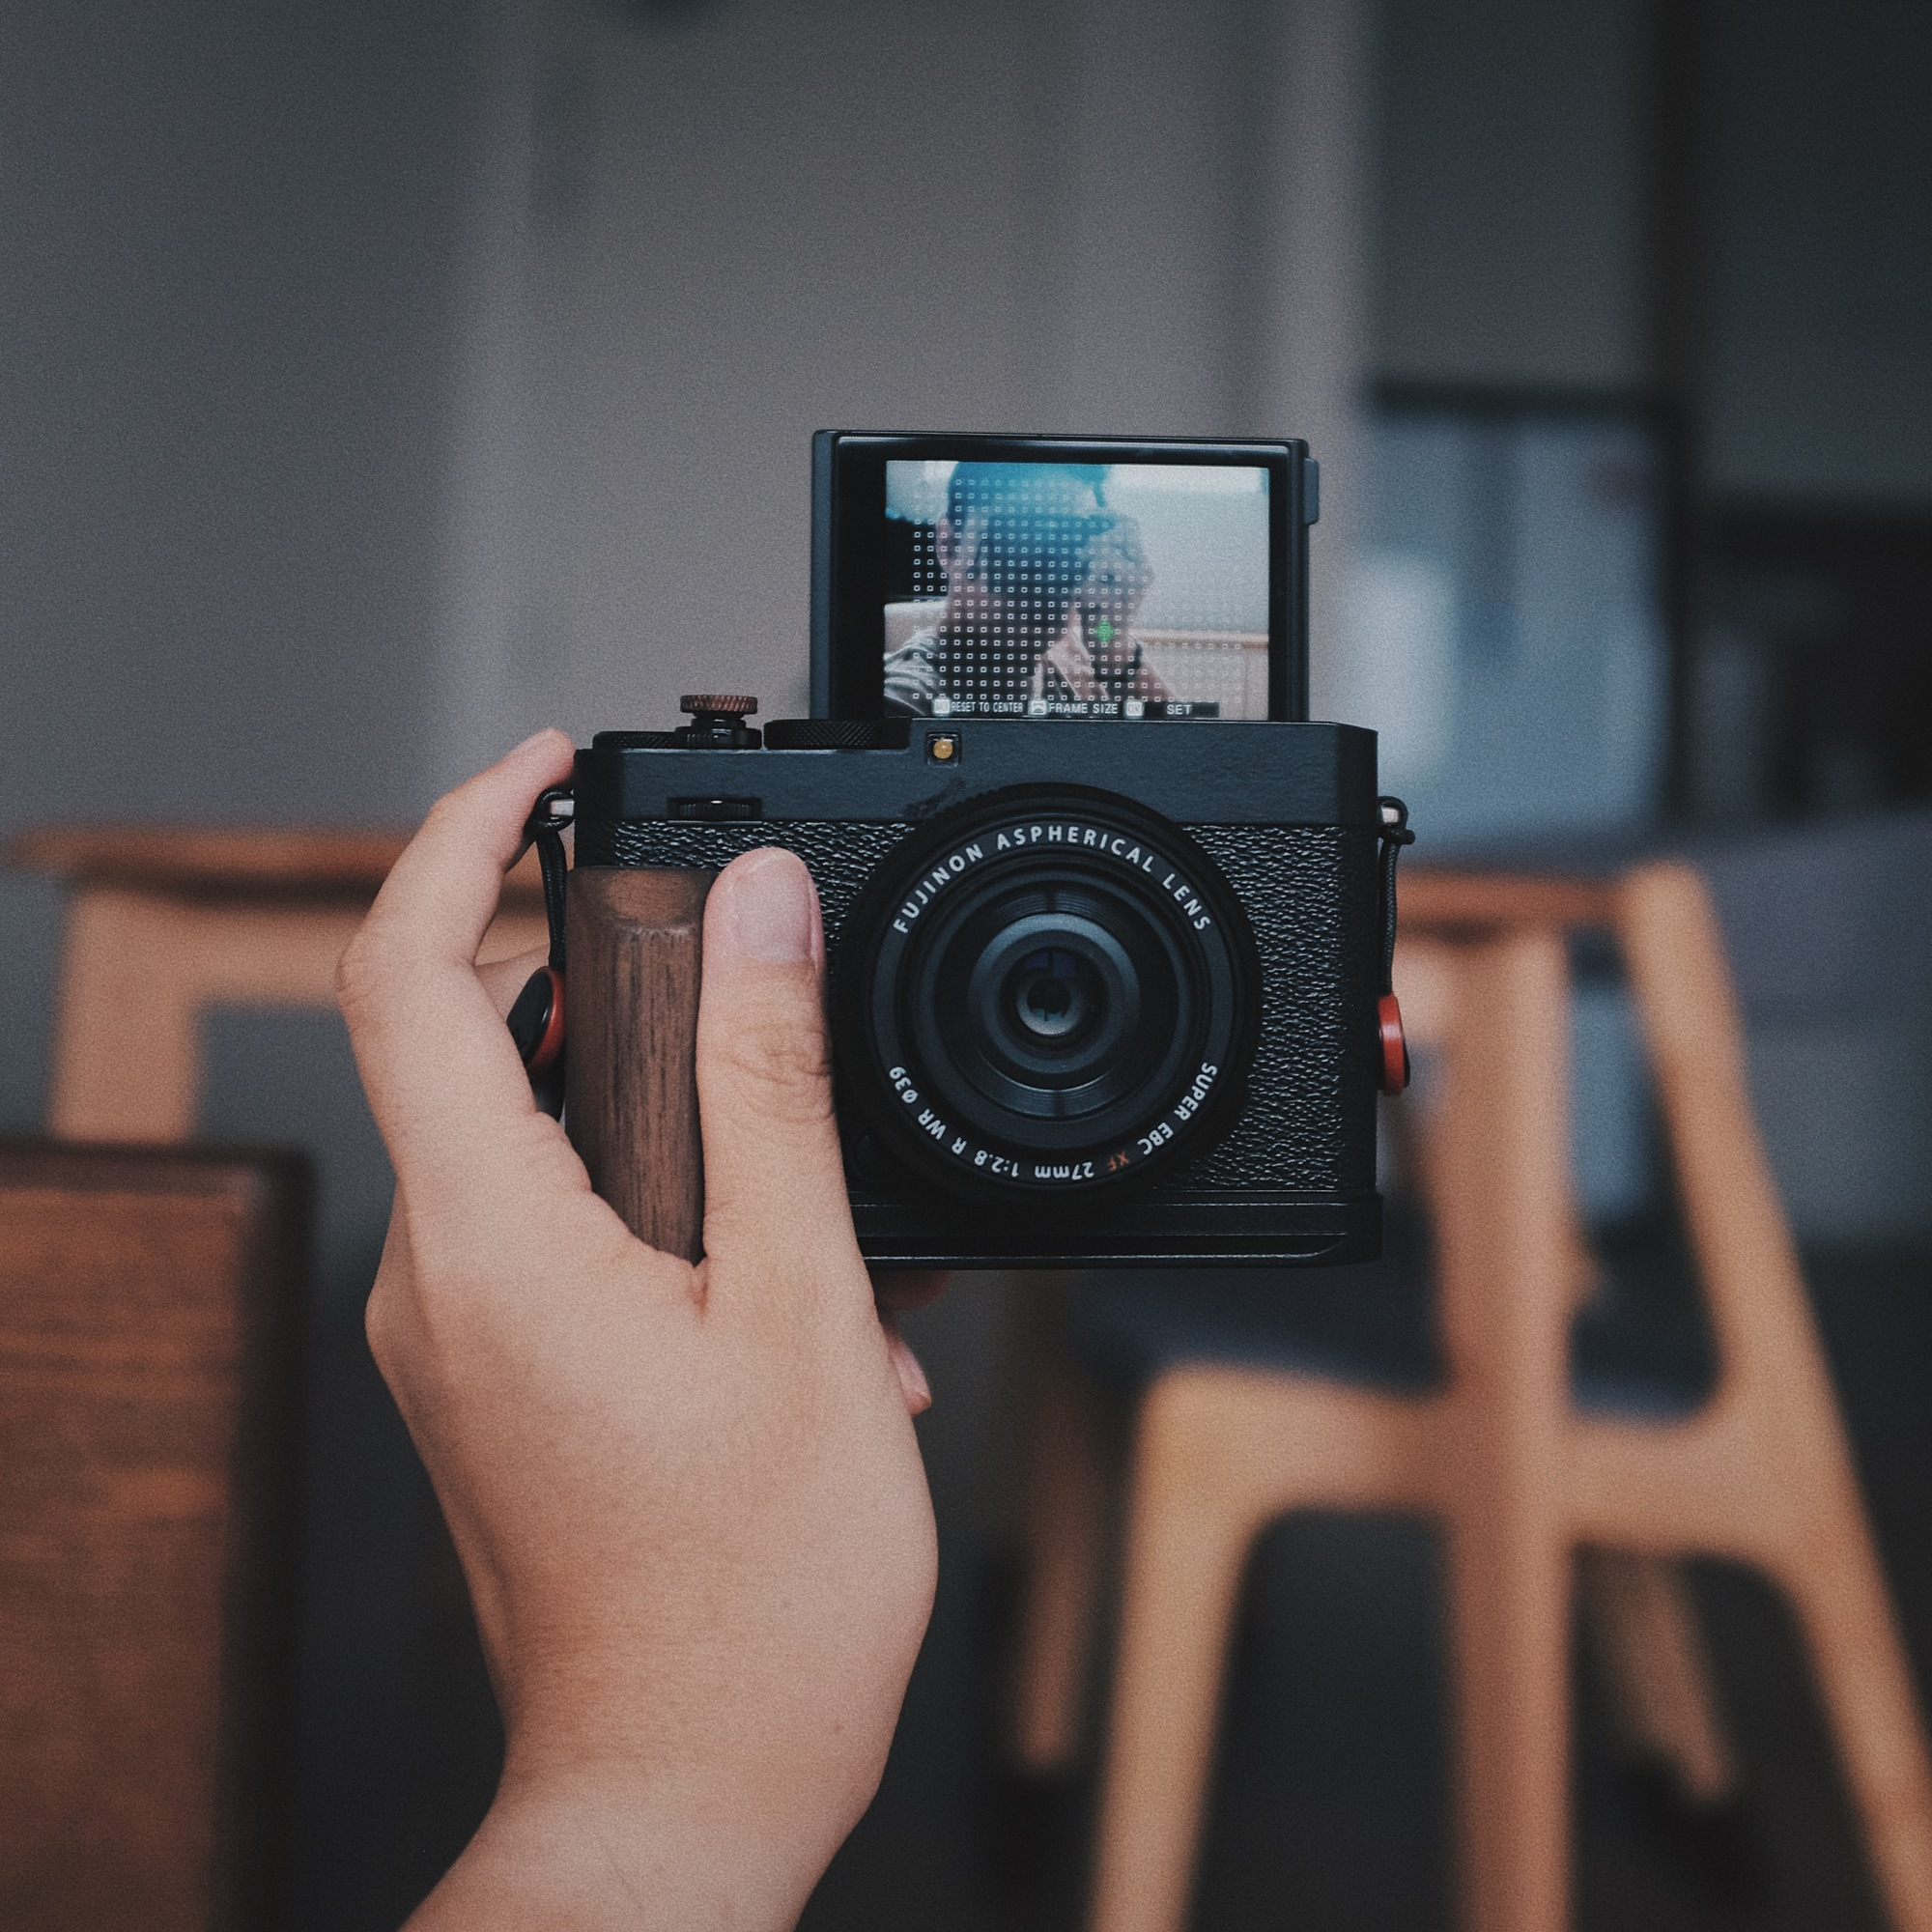
\includegraphics[width=\linewidth]{\envfinaldir/coverpic-prod.jpg}\par
            % \vskip 30pt
            \vfill

            \normalsize\rmfamily\scshape
            \copyright{} The Web Digest Project \hfill\large \envdatestr
        \end{center}
    \end{titlepage}
    % \restoregeometry
}
\newcommand{\simplehref}[1]{%
    \textcolor{blue!80!green}{\href{#1}{#1}}%
}
\renewcommand{\contentsname}{\center\Huge\sffamily\bfseries Contents\par\vskip 20pt}
\newcounter{ipartcounter}
\setcounter{ipartcounter}{0}
\newcommand{\ipart}[1]{
    % \vskip 20pt
    \clearpage
    \stepcounter{ipartcounter}
    \phantomsection
    \addcontentsline{toc}{chapter}{#1}
    % \begin{center}
    %     \Huge
    %     \sffamily\bfseries
    %     #1
    % \end{center}
    % \vskip 20pt plus 7pt
}
\newcounter{ichaptercounter}
\setcounter{ichaptercounter}{0}
\newcommand{\ichapter}[1]{
    % \vskip 20pt
    \clearpage
    \stepcounter{ichaptercounter}
    \phantomsection
    \addcontentsline{toc}{section}{\numberline{\arabic{ichaptercounter}}#1}
    \begin{center}
        \Huge
        \sffamily\bfseries
        #1
    \end{center}
    \vskip 20pt plus 7pt
}
\newcommand{\entrytitlefont}[1]{\subsection*{\raggedright\Large\sffamily\bfseries#1}}
\newcommand{\entryitemGeneric}[2]{
    % argv: title, url
    \parbox{\linewidth}{
        \entrytitlefont{#1}\par\vskip 5pt
        \footnotesize\ttfamily\mdseries
        \simplehref{#2}
    }\vskip 11pt plus 11pt minus 1pt
}
\newcommand{\entryitemGithub}[3]{
    % argv: title, url, desc
    \parbox{\linewidth}{
        \entrytitlefont{#1}\par\vskip 5pt
        \footnotesize\ttfamily\mdseries
        \simplehref{#2}\par\vskip 5pt
        \small\rmfamily\mdseries#3
    }\vskip 11pt plus 11pt minus 1pt
}
\newcommand{\entryitemAp}[3]{
    % argv: title, url, desc
    \parbox{\linewidth}{
        \entrytitlefont{#1}\par\vskip 5pt
        \footnotesize\ttfamily\mdseries
        \simplehref{#2}\par\vskip 5pt
        \small\rmfamily\mdseries#3
    }\vskip 11pt plus 11pt minus 1pt
}
\newcommand{\entryitemHackernews}[3]{
    % argv: title, hnurl, rawurl
    % \parbox{\linewidth}{
    %     \entrytitlefont{#1}\par\vskip 5pt
    %     \footnotesize\ttfamily\mdseries
    %     \simplehref{#3}\par
    %     \textcolor{black!50}{\href{#2}{#2}}
    % }\vskip 11pt plus 11pt minus 1pt
    \begin{minipage}{\linewidth}
            \entrytitlefont{#1}\par\vskip 5pt
            \footnotesize\ttfamily\mdseries
            \simplehref{#3}\par
            \textcolor{black!50}{\href{#2}{#2}}
    \end{minipage}\par\vskip 11pt plus 11pt minus 1pt
}







\begin{document}

\makeheader

\tableofcontents\clearpage




\ipart{Developers}
\ichapter{Hacker News}
\entryitemTwoLinks{AI Demos}{https://news.ycombinator.com/item?id=42992643}{https://aidemos.meta.com/}

\entryitemTwoLinks{Why Blog If Nobody Reads It?}{https://news.ycombinator.com/item?id=42992159}{https://andysblog.uk/why-blog-if-nobody-reads-it/}

\entryitemTwoLinks{UnitedHealth Is Sick of Everyone Complaining About Its Claim Denials}{https://news.ycombinator.com/item?id=42992121}{https://www.rollingstone.com/culture/culture-news/unitedhealth-defends-image-claim-denials-mangione-thompson-1235259054/}

\entryitemTwoLinks{LIMO: Less Is More for Reasoning}{https://news.ycombinator.com/item?id=42991676}{https://arxiv.org/abs/2502.03387}

\entryitemTwoLinks{Kanata: Cross-platform multi-layer keyboard remapper with advanced customization}{https://news.ycombinator.com/item?id=42991019}{https://github.com/jtroo/kanata}

\entryitemTwoLinks{Hard disk fraud: long runtimes on new Seagate hard disks}{https://news.ycombinator.com/item?id=42991006}{https://www.heise.de/en/news/Hard-disk-fraud-Increasing-evidence-of-origin-in-China-10269059.html}

\entryitemTwoLinks{Baffled by generational garbage collection – wingolog}{https://news.ycombinator.com/item?id=42990819}{https://wingolog.org/archives/2025/02/09/baffled-by-generational-garbage-collection}

\entryitemTwoLinks{Don't "optimize" conditional moves in shaders with mix()+step()}{https://news.ycombinator.com/item?id=42990324}{https://iquilezles.org/articles/gpuconditionals/}

\entryitemTwoLinks{Classic Data science pipelines built with LLMs}{https://news.ycombinator.com/item?id=42990036}{https://github.com/Pravko-Solutions/FlashLearn/tree/main/examples}

\entryitemTwoLinks{Dear Mr. Vice President, Please Take Off Your Apple Watch}{https://news.ycombinator.com/item?id=42990000}{https://www.watchesofespionage.com/blogs/woe-dispatch/vice-president-jd-vance-apple-watch-smartwatch-intelligence-risks}

\entryitemTwoLinks{RetroFab: Playable 3D simulations of vintage electronic games}{https://news.ycombinator.com/item?id=42989628}{https://itizso.itch.io/retrofab}

\entryitemTwoLinks{Mathematics in the 20th century, by Michael Atiyah [pdf] (2002)}{https://news.ycombinator.com/item?id=42989419}{https://marktomforde.com/academic/miscellaneous/images/atiyah20thcentury.pdf}

\entryitemTwoLinks{Modern-Day Oracles or Bullshit Machines? How to thrive in a ChatGPT world}{https://news.ycombinator.com/item?id=42989320}{https://thebullshitmachines.com}

\entryitemTwoLinks{Brain Hyperconnectivity in Children with Autism and Its Links to Social Deficits (2013)}{https://news.ycombinator.com/item?id=42988303}{https://www.cell.com/cell-reports/fulltext/S2211-1247(13)00570-6}

\entryitemTwoLinks{Is software abstraction killing civilization? (2021)}{https://news.ycombinator.com/item?id=42986485}{https://datagubbe.se/endofciv/}

\entryitemTwoLinks{Jacksonpollock.org (2003)}{https://news.ycombinator.com/item?id=42986320}{https://jacksonpollock.org/}

\entryitemTwoLinks{Tips for mathematical handwriting (2007)}{https://news.ycombinator.com/item?id=42985427}{https://johnkerl.org/doc/ortho/ortho.html}

\entryitemTwoLinks{Rwandan scientists develop local yeast for banana wine-makers}{https://news.ycombinator.com/item?id=42985342}{https://phys.org/news/2025-01-rwandan-scientists-local-yeast-banana.html}

\entryitemTwoLinks{Writing a simple windows driver in Rust}{https://news.ycombinator.com/item?id=42984457}{https://scorpiosoftware.net/2025/02/08/writing-a-simple-driver-in-rust/}

\entryitemTwoLinks{Show HN: FlashSpace – fast, open-source, macOS Spaces replacement}{https://news.ycombinator.com/item?id=42984420}{https://github.com/wojciech-kulik/FlashSpace}\ichapter{Phoronix}
\entryitemGeneric{\hskip 0pt{}Linux 6.14-rc2 Released With Apple Silicon Maintainer Change, Bcachefs Fixes}{https://www.phoronix.com/news/Linux-6.14-rc2-Released}

\entryitemGeneric{\hskip 0pt{}Linux Patches Adjust AC Plug/Unplug Behavior During s2idle To Match Windows}{https://www.phoronix.com/news/Linux-Patches-AC-Plug-s2idle}

\entryitemGeneric{\hskip 0pt{}Curious Intel Linux Driver Maintainer Changes In Recent Days}{https://www.phoronix.com/news/Intel-Linux-Maintainer-Changes}

\entryitemGeneric{\hskip 0pt{}Intel ISPC 1.26 Compiler Delivers Improved ARM Support}{https://www.phoronix.com/news/Intel-ISPC-1.26}

\entryitemGeneric{\hskip 0pt{}New Apple Silicon Co-Maintainer Steps Up For The Linux Kernel}{https://www.phoronix.com/news/Apple-Silicon-New-Co-Maintainer}

\entryitemGeneric{\hskip 0pt{}Linux FineIBT-BHI Updated For Toughening Up FineIBT Kernel Defenses}{https://www.phoronix.com/news/Linux-FineIBT-BHI-Linux-2025}

\entryitemGeneric{\hskip 0pt{}Wine-Staging 10.1 Delivers 361 Patches Atop Upstream Wine}{https://www.phoronix.com/news/Wine-Staging-10.1-Released}

\entryitemGeneric{\hskip 0pt{}SysVinit 3.14 Released: Overcomes Three Decade Limitation Of Inittab Line Length}{https://www.phoronix.com/news/SysVinit-3.14-Released}

\entryitemGeneric{\hskip 0pt{}Clang Thread Safety Checks Begin Uncovering Bugs In The Linux Kernel}{https://www.phoronix.com/news/Linux-Clang-Thread-Safety}\ichapter{Dribbble}
\entryitemGeneric{\hskip 0pt{}Barbershop POS app for booking and payments}{https://dribbble.com/shots/25596116-Barbershop-POS-app-for-booking-and-payments}

\entryitemGeneric{\hskip 0pt{}Seam Logo Redesigned}{https://dribbble.com/shots/25595119-Seam-Logo-Redesigned}

\entryitemGeneric{\hskip 0pt{}Nimmio}{https://dribbble.com/shots/25594035-Nimmio}

\entryitemGeneric{\hskip 0pt{}Cloaked Logo Design}{https://dribbble.com/shots/25585116-Cloaked-Logo-Design}

\entryitemGeneric{\hskip 0pt{}The Journey}{https://dribbble.com/shots/25590279-The-Journey}

\entryitemGeneric{\hskip 0pt{}CropBytes 2d \& 3d logo}{https://dribbble.com/shots/25590388-CropBytes-2d-3d-logo}

\entryitemGeneric{\hskip 0pt{}Wylder Logo Design - W letter monogram}{https://dribbble.com/shots/25589195-Wylder-Logo-Design-W-letter-monogram}

\entryitemGeneric{\hskip 0pt{}Tailor Brands Logo}{https://dribbble.com/shots/25590868-Tailor-Brands-Logo}

\entryitemGeneric{\hskip 0pt{}Carbon Solutions B2B Branding Design \& Visual Identity}{https://dribbble.com/shots/25525140-Carbon-Solutions-B2B-Branding-Design-Visual-Identity}

\entryitemGeneric{\hskip 0pt{}Dog / Puzzle Logo}{https://dribbble.com/shots/25581316-Dog-Puzzle-Logo}

\entryitemGeneric{\hskip 0pt{}Frank's Alley® Trailer \& Mascots}{https://dribbble.com/shots/25585516-Frank-s-Alley-Trailer-Mascots}

\entryitemGeneric{\hskip 0pt{}Glyph Beer Icons 51-62}{https://dribbble.com/shots/25585199-Glyph-Beer-Icons-51-62}

\entryitemGeneric{\hskip 0pt{}Realtree® 30 Years.}{https://dribbble.com/shots/25579343-Realtree-30-Years}

\entryitemGeneric{\hskip 0pt{}VCC Logo Design Vector Sketches}{https://dribbble.com/shots/25577220-VCC-Logo-Design-Vector-Sketches}

\entryitemGeneric{\hskip 0pt{}Brand Family System Loop}{https://dribbble.com/shots/25579103-Brand-Family-System-Loop}

\entryitemGeneric{\hskip 0pt{}Chilbot Motion Design}{https://dribbble.com/shots/25578623-Chilbot-Motion-Design}

\entryitemGeneric{\hskip 0pt{}Weve Branding}{https://dribbble.com/shots/25579635-Weve-Branding}

\entryitemGeneric{\hskip 0pt{}S}{https://dribbble.com/shots/25571540-S}

\entryitemGeneric{\hskip 0pt{}Fly Fry}{https://dribbble.com/shots/25573635-Fly-Fry}

\entryitemGeneric{\hskip 0pt{}Logo and Branding for VCC}{https://dribbble.com/shots/25571598-Logo-and-Branding-for-VCC}

\entryitemGeneric{\hskip 0pt{}Axolotl Mascot}{https://dribbble.com/shots/25572670-Axolotl-Mascot}

\entryitemGeneric{\hskip 0pt{}TIAA Duotone Icons}{https://dribbble.com/shots/25573874-TIAA-Duotone-Icons}

\entryitemGeneric{\hskip 0pt{}Finance APP UI Design}{https://dribbble.com/shots/25570740-Finance-APP-UI-Design}

\entryitemGeneric{\hskip 0pt{}Cloud Animation Sound Design}{https://dribbble.com/shots/25571319-Cloud-Animation-Sound-Design}


\ipart{Developers~~~~(zh-Hans)}
\ichapter{Solidot}
\entryitemGeneric{\hskip 0pt{}萨尔瓦多议会投票撤销比特币的法币地位}{https://www.solidot.org/story?sid=80510}

\entryitemGeneric{\hskip 0pt{}消费者对微软力推的 Copilot+ PC 缺乏兴趣}{https://www.solidot.org/story?sid=80509}

\entryitemGeneric{\hskip 0pt{}强太阳风暴之后地球周围观察到神秘辐射带}{https://www.solidot.org/story?sid=80508}

\entryitemGeneric{\hskip 0pt{}美国科技巨头加大力度投资 AI 数据中心}{https://www.solidot.org/story?sid=80507}

\entryitemGeneric{\hskip 0pt{}僵尸设备成为日益严重的网络安全风险}{https://www.solidot.org/story?sid=80506}

\entryitemGeneric{\hskip 0pt{}日本三孩以上家庭将免学费上大学}{https://www.solidot.org/story?sid=80505}

\entryitemGeneric{\hskip 0pt{}波音在 Starliner 项目上总损失超过了 20 亿美元}{https://www.solidot.org/story?sid=80504}

\entryitemGeneric{\hskip 0pt{}法国铁路对开扬声器打电话的乘客罚款 150 欧元}{https://www.solidot.org/story?sid=80503}

\entryitemGeneric{\hskip 0pt{}印度将推出银行专用域名 .bank.in}{https://www.solidot.org/story?sid=80502}

\entryitemGeneric{\hskip 0pt{}Microsoft 365 订阅费用准备涨价}{https://www.solidot.org/story?sid=80501}

\entryitemGeneric{\hskip 0pt{}Meta 从盗版电子书库下载了逾百 TB 的电子书}{https://www.solidot.org/story?sid=80500}

\entryitemGeneric{\hskip 0pt{}由于维护者拒绝 DMA Rust 抽象 Hector Martin 宣布退出内核开发}{https://www.solidot.org/story?sid=80499}

\entryitemGeneric{\hskip 0pt{}扩展开发者称 Google 没有信守在宣布 Manifest V3 时许下的承诺}{https://www.solidot.org/story?sid=80498}

\entryitemGeneric{\hskip 0pt{}英国政府命令苹果创建 iCloud 加密后门}{https://www.solidot.org/story?sid=80497}

\entryitemGeneric{\hskip 0pt{}Goolge 修复正被利用的 Android 内核 0day 漏洞}{https://www.solidot.org/story?sid=80496}

\entryitemGeneric{\hskip 0pt{}相信外星人的上世纪硅谷高管面临监禁}{https://www.solidot.org/story?sid=80495}

\entryitemGeneric{\hskip 0pt{}科学家声称找到煮鸡蛋的完美方法}{https://www.solidot.org/story?sid=80494}

\entryitemGeneric{\hskip 0pt{}2024 年勒索软件付款额下降 35\%}{https://www.solidot.org/story?sid=80493}

\entryitemGeneric{\hskip 0pt{}美国分析师认为 DeepSeek 的 AI App 有很高的可能性被禁}{https://www.solidot.org/story?sid=80492}

\entryitemGeneric{\hskip 0pt{}空气污染会影响日常工作的专注力}{https://www.solidot.org/story?sid=80491}\ichapter{V2EX}
\entryitemGeneric{\hskip 0pt{}[程序员] FilePulse 一款高效搜索工具。支持中文搜索,拼音搜索,拼音首字母搜索。文件夹的大小将自动实时计算,支持 HTTP2/HTTP3。}{https://www.v2ex.com/t/1110175}

\entryitemGeneric{\hskip 0pt{}[NAS] 铁威马 D4-320 硬盘柜如何配电源}{https://www.v2ex.com/t/1110173}

\entryitemGeneric{\hskip 0pt{}[生活] 回家吧,不要再纠结了。}{https://www.v2ex.com/t/1110172}

\entryitemGeneric{\hskip 0pt{}[酷工作] AI 前端实习生(远程)}{https://www.v2ex.com/t/1110170}

\entryitemGeneric{\hskip 0pt{}[酷工作] AI 前端/全栈工程师(远程)}{https://www.v2ex.com/t/1110169}

\entryitemGeneric{\hskip 0pt{}[分享创造] 一个用抽象层来管理数据库的 mcp 服务 mcp-dbutils}{https://www.v2ex.com/t/1110168}

\entryitemGeneric{\hskip 0pt{}[NAS] 台式机做 nas 可行吗}{https://www.v2ex.com/t/1110167}

\entryitemGeneric{\hskip 0pt{}[分享发现] 图书馆期刊室可看的计算机期刊学报}{https://www.v2ex.com/t/1110166}

\entryitemGeneric{\hskip 0pt{}[GitHub Copilot] 曾经的王者 Copilot 这算是追上 Cursor 了吗?}{https://www.v2ex.com/t/1110164}

\entryitemGeneric{\hskip 0pt{}[深圳] 打算上半年学个车,有什么要避坑的吗,坐标深圳}{https://www.v2ex.com/t/1110163}

\entryitemGeneric{\hskip 0pt{}[问与答] 有没有鼠标放上去 即可朗读单词的网页插件}{https://www.v2ex.com/t/1110162}

\entryitemGeneric{\hskip 0pt{}[Java] 在 GitHub 下载的 program,无法登录}{https://www.v2ex.com/t/1110161}

\entryitemGeneric{\hskip 0pt{}[CSS] Chrome 133.0.6943.60 @media (pointer: fine) 失效?}{https://www.v2ex.com/t/1110159}

\entryitemGeneric{\hskip 0pt{}[问与答] 夸克网盘这个问题是怎么回事?}{https://www.v2ex.com/t/1110158}

\entryitemGeneric{\hskip 0pt{}[酷工作] [北京] Web3 公司招聘 Python 开发工程师,可远程[20-26K]}{https://www.v2ex.com/t/1110157}

\entryitemGeneric{\hskip 0pt{}[iPad] 苹果砍掉 11 寸设备的拆分键盘之后,自己实现了拆分键盘的输入法有哪些?}{https://www.v2ex.com/t/1110156}

\entryitemGeneric{\hskip 0pt{}[Linux] 从进程到协程:计算机的并发编程之路}{https://www.v2ex.com/t/1110155}

\entryitemGeneric{\hskip 0pt{}[微信] 国外手机号注册的 WeChat 能使用网页微信吗?}{https://www.v2ex.com/t/1110154}

\entryitemGeneric{\hskip 0pt{}[问与答] 在 JD 线下门店使用国补用 7199 买了 Macbook Air M3 24+512,比 JD 网上便宜 800}{https://www.v2ex.com/t/1110153}

\entryitemGeneric{\hskip 0pt{}[奇思妙想] 有了 AI,开发门槛降低,但独立开发者并不等于只需要开发就能挣钱}{https://www.v2ex.com/t/1110152}

\entryitemGeneric{\hskip 0pt{}[程序员] DeepSeek``服务器繁忙''解决方案(饮鸩止渴版)}{https://www.v2ex.com/t/1110151}

\entryitemGeneric{\hskip 0pt{}[程序员] cursor 中使用 powershell 跳出一大堆路径}{https://www.v2ex.com/t/1110150}

\entryitemGeneric{\hskip 0pt{}[NAS] Nas 读写文件速度奇慢无比,排错了半天,最终。。。。。}{https://www.v2ex.com/t/1110148}

\entryitemGeneric{\hskip 0pt{}[问与答] 现在还有人自己建站搭建博客吃广告费吗?}{https://www.v2ex.com/t/1110147}

\entryitemGeneric{\hskip 0pt{}[Android] 安卓是否有开源系统可通过两个不同解锁密码,启用两个都可的安卓系统啊?}{https://www.v2ex.com/t/1110146}

\entryitemGeneric{\hskip 0pt{}[旅行] 想自驾游,求指导}{https://www.v2ex.com/t/1110145}

\entryitemGeneric{\hskip 0pt{}[Apple] 手持 iPad Pro 11 寸 A12Z 处理器 是否有必要换新款 iPad Pro 了}{https://www.v2ex.com/t/1110143}

\entryitemGeneric{\hskip 0pt{}[广州] 广州越秀合租| 1200 主卧找室友,近地铁 1 号}{https://www.v2ex.com/t/1110142}

\entryitemGeneric{\hskip 0pt{}[生活] 696 天,分手了}{https://www.v2ex.com/t/1110139}

\entryitemGeneric{\hskip 0pt{}[问与答] 甘肃兰州有啥工作推荐吗?}{https://www.v2ex.com/t/1110138}

\entryitemGeneric{\hskip 0pt{}[问与答] 收到微信登录验证码短信,是诈骗吗?}{https://www.v2ex.com/t/1110136}

\entryitemGeneric{\hskip 0pt{}[问与答] 作为个人想弄个认证的企业微信,有什么办法吗?}{https://www.v2ex.com/t/1110133}

\entryitemGeneric{\hskip 0pt{}[酷工作] [招聘] 帮朋友发石家庄 C/C++通信类软件开发岗招聘}{https://www.v2ex.com/t/1110131}

\entryitemGeneric{\hskip 0pt{}[互联网] 人类依赖 AI 会不会退化?}{https://www.v2ex.com/t/1110129}

\entryitemGeneric{\hskip 0pt{}[日本] 北京 | 男 | 清明日本关西旅游 | 寻队友}{https://www.v2ex.com/t/1110127}

\entryitemGeneric{\hskip 0pt{}[职场话题] 快 27 岁了,想试试客户面的工作}{https://www.v2ex.com/t/1110126}

\entryitemGeneric{\hskip 0pt{}[程序员] 人生第一个国补 M3 Macbook Air 24+512}{https://www.v2ex.com/t/1110125}

\entryitemGeneric{\hskip 0pt{}[北京] 出租\_西二旗融泽嘉园小区房东直租}{https://www.v2ex.com/t/1110124}

\entryitemGeneric{\hskip 0pt{}[职场话题] 双方都在互联网大厂的程序员夫妻,攒钱真迅猛。}{https://www.v2ex.com/t/1110123}

\entryitemGeneric{\hskip 0pt{}[分享创造] 分享一篇交互式魔方复原博客}{https://www.v2ex.com/t/1110121}

\entryitemGeneric{\hskip 0pt{}[生活] V 友的实际年龄和身份证年龄一样吗?}{https://www.v2ex.com/t/1110120}

\entryitemGeneric{\hskip 0pt{}[输入法] 求解: macOS 下搜狗输入法在终端输入时按 Shift 总出现多余字符}{https://www.v2ex.com/t/1110118}

\entryitemGeneric{\hskip 0pt{}[阅读] zlibrary 网站用不了了}{https://www.v2ex.com/t/1110117}

\entryitemGeneric{\hskip 0pt{}[iPhone] 未来美版有锁即将成为历史}{https://www.v2ex.com/t/1110116}

\entryitemGeneric{\hskip 0pt{}[Apple] 求推荐稍后阅读的 app}{https://www.v2ex.com/t/1110114}

\entryitemGeneric{\hskip 0pt{}[问与答] iPod 导入歌曲}{https://www.v2ex.com/t/1110113}

\entryitemGeneric{\hskip 0pt{}[奇思妙想] 随想:人所以为人,是因为人会用工具!}{https://www.v2ex.com/t/1110112}

\entryitemGeneric{\hskip 0pt{}[科技] ios 有类似 cherry studio 这样的应用吗}{https://www.v2ex.com/t/1110111}

\entryitemGeneric{\hskip 0pt{}[Android] 2025 年 pixel 安卓玩机方案?}{https://www.v2ex.com/t/1110110}

\entryitemGeneric{\hskip 0pt{}[程序员] 我怎么感觉现在, AI 对编程的辅助,并没有网上讨论的那样夸张}{https://www.v2ex.com/t/1110109}


\ipart{Generic News}
\ichapter{AP News}
\entryitemWithDescription{\hskip 0pt{}Trump says he is serious about Canada becoming 51st state in Super Bowl interview}{https://apnews.com/article/7e1959c7d430899b01629c800db6f17b}{}

\entryitemWithDescription{\hskip 0pt{}Sam Nujoma, Namibia's fiery freedom fighter and first president, dies aged 95}{https://apnews.com/article/290a2392f311408498f4734d14c69918}{}

\entryitemWithDescription{\hskip 0pt{}Post Malone, Travis Scott, Latto perform at star-studded, invite-only Fanatics Super Bowl party}{https://apnews.com/article/fb63e81d72143c5b690afc6cd04287ae}{}

\entryitemWithDescription{\hskip 0pt{}Hawaii is the rainbow capital of the world. Here's what that means}{https://apnews.com/article/f9498854a95de626905627602ac90d87}{}

\entryitemWithDescription{\hskip 0pt{}Dalai Lama's elder brother, who led several rounds of talks with China, dies at 97}{https://apnews.com/article/1459f99b6cf1c342919ad195fd27fa33}{}

\entryitemWithDescription{\hskip 0pt{}Du Plessis successfully defends middleweight belt in rematch with Strickland in UFC 312}{https://apnews.com/article/46d167c1fa1a9ec912bef596b9e530e2}{}

\entryitemWithDescription{\hskip 0pt{}Call it the Dog Bowl. Westminster show's canine athletes get their piece of Super Bowl weekend}{https://apnews.com/article/dc6adab062addc923d381c2dce97ba56}{}

\entryitemWithDescription{\hskip 0pt{}He's back, baby! ESPN's Dick Vitale makes return to commentating following 4th bout with cancer}{https://apnews.com/article/c8ae64fb1d7b602b1874f4a1080d8012}{}

\entryitemWithDescription{\hskip 0pt{}Longtime NFL player and coach Dick Jauron dies at 74}{https://apnews.com/article/0abb2c30f8dbb33e85e22159799c93a9}{}

\entryitemWithDescription{\hskip 0pt{}Nelly delivers hits at `Homecoming' Super Bowl week concert in historic New Orleans restaurant}{https://apnews.com/article/003099c9fa33ccb82b8b2e6f7533ffdd}{}

\entryitemWithDescription{\hskip 0pt{}It's a girl! Sweden's Prince Carl Philip and Princess Sofia announce birth of their first daughter}{https://apnews.com/article/723e61d04df87902f42b98cee155c1ff}{}

\entryitemWithDescription{\hskip 0pt{}At 72 years old and out of the NFL, Bill Belichick makes presence known at the Super Bowl}{https://apnews.com/article/d9cf9f554a9524196d1716addc1078c9}{}

\entryitemWithDescription{\hskip 0pt{}`It looks like a stream of blood.' A river near Buenos Aires turns red, sparking fears of toxic leak}{https://apnews.com/article/41a713c0ecdadadf204c330465a3f7e9}{}\ichapter{Reuters}
\entryitemWithDescription{\hskip 0pt{}Russia awaits appropriate signals from US on contacts, senior diplomat says}{https://www.reuters.com/world/russia-awaits-appropriate-signals-us-contacts-senior-diplomat-says-2025-02-09/}{Russian envoy to the United Nations, in remarks published on Sunday, said Russia was waiting for "appropriate signals" from Washington on contacts with Moscow, but he had few expectations for better ties with Washington\textquotesingle s...}

\entryitemWithDescription{\hskip 0pt{}Trump says he is committed to US ownership of Gaza}{https://www.reuters.com/world/middle-east/trump-says-he-is-committed-us-ownership-gaza-2025-02-09/}{U.S. President Donald Trump on Sunday said that he is committed to buying and owning Gaza, but could give sections of the land to other states in the Middle East to help in the rebuilding...}

\entryitemWithDescription{\hskip 0pt{}Egypt disapproves of statements by Netanyahu in US media, foreign ministry says}{https://www.reuters.com/world/egypt-disapproves-statements-by-netanyahu-us-media-foreign-ministry-says-2025-02-09/}{Egypt disapproves of the statements made by Israeli Prime Minister Benjamin Netanyahu in U.S. media describing them as "misleading accusations", the foreign ministry said late on...}

\entryitemWithDescription{\hskip 0pt{}Afghans who worked with US should be exempt from aid, refugee freeze, advocacy group says}{https://www.reuters.com/world/us/afghans-who-worked-with-us-should-be-exempt-aid-refugee-freeze-advocacy-group-2025-02-09/}{A group representing U.S. veterans, service members and others is warning the Trump administration of severe impacts on U.S. security unless it exempts tens of thousands of Afghans -- many at risk of Taliban retribution -- from the...}

\entryitemWithDescription{\hskip 0pt{}German Chancellor candidates clash on Trump, the far-right and NATO}{https://www.reuters.com/world/europe/europe-can-act-within-an-hour-if-us-levies-tariffs-germanys-scholz-2025-02-09/}{Europe is prepared to respond "within an hour" if the United States levies tariffs against the European Union, German Chancellor Olaf Scholz said in a pre-election debate with his conservative challenger Friedrich...}

\entryitemWithDescription{\hskip 0pt{}Dozens of runaway Congo soldiers face trial on violence charges}{https://www.reuters.com/world/africa/dozens-runaway-congo-soldiers-face-trial-violence-charges-2025-02-09/}{Congo authorities will put at least 75 soldiers on trial on Monday for fleeing the advance of Rwanda-backed M23 rebels into the eastern province of South Kivu and for violence against civilians, including murder and looting, the military...}

\entryitemWithDescription{\hskip 0pt{}Trump plan to end Ukraine war must prevent new Russian aggression, Zelenskiy says}{https://www.reuters.com/world/europe/ukraines-zelenskiy-trump-plan-must-not-only-end-war-prevent-new-russian-2025-02-09/}{Zelenskiy again ruled out holding elections in Ukraine until hostilities...}

\entryitemWithDescription{\hskip 0pt{}Colombia's environment minister resigns, stays on as COP16 head}{https://www.reuters.com/world/americas/colombias-environment-minister-resigns-stays-cop16-head-2025-02-09/}{Colombia\textquotesingle s Environment Minister Susana Muhamad said on Sunday she has informed President Gustavo Petro of her resignation from the...}

\entryitemWithDescription{\hskip 0pt{}Trump to meet with leaders of Saudi Arabia and Egypt, Israeli president says}{https://www.reuters.com/world/trump-meet-with-leaders-saudi-arabia-egypt-israeli-president-says-2025-02-09/}{Israeli President Isaac Herzog said on Sunday that U.S. President Donald Trump was set to meet with Egyptian President Abdel Fattah el-Sisi and possibly Saudi Arabian Crown Prince Mohammed bin Salman, although he gave no dates for the...}

\entryitemWithDescription{\hskip 0pt{}Chief of violence-hit Indian state of Manipur resigns}{https://www.reuters.com/world/india/chief-violence-hit-indian-state-manipur-resigns-2025-02-09/}{The chief minister of India\textquotesingle s northeastern state of Manipur resigned on Sunday, bowing to pressure to quit amid ongoing ethnic clashes that have cost at least 250 lives since they broke out nearly two years...}

\entryitemWithDescription{\hskip 0pt{}South Africa's land act targets a stark divide, Trump and Musk oppose it}{https://www.reuters.com/world/stark-divide-that-south-africas-land-act-seeks-bridge-2025-02-09/}{A law that allows the government to confiscate land has reignited racial tensions that have dogged Africa\textquotesingle s southernmost tip ever since European settlers began arriving nearly four centuries...}

\entryitemWithDescription{\hskip 0pt{}'No thanks': White South Africans turn down Trump's immigration offer}{https://www.reuters.com/world/africa/no-thanks-white-south-africans-turn-down-trumps-immigration-offer-2025-02-09/}{The ANC says Trump is amplifying misinformation propagated by an Afrikaner-led...}

\entryitemWithDescription{\hskip 0pt{}Baltic states switch to European power grid, ending Russia ties}{https://www.reuters.com/business/energy/baltic-states-switch-european-power-grid-ending-russia-ties-2025-02-09/}{The Baltic states of Estonia, Latvia and Lithuania completed a switch from Russia\textquotesingle s electricity grid to the EU\textquotesingle s system on Sunday, severing Soviet-era ties amid heightened security after the suspected...}






\clearpage
\leavevmode\vfill
\footnotesize

Copyright \copyright{} 2023-2025 Neruthes and other contributors.

This document is published with CC BY-NC-ND 4.0 license.

The entries listed in this newsletter may be copyrighted by their respective creators.

This newsletter is generated by the Web Digest project.

The newsletters are also delivered via Telegram channel \CJKunderline{\href{https://t.me/webdigestchannel}{https://t.me/webdigestchannel}}.\\
RSS feed is available at \CJKunderline{\href{https://webdigest.pages.dev/rss.xml}{https://webdigest.pages.dev/rss.xml}}.

This newsletter is available in PDF at
\CJKunderline{\href{https://webdigest.pages.dev/}{https://webdigest.pages.dev/}}.

The source code being used to generate this newsletter is available at\\
\CJKunderline{\href{https://github.com/neruthes/webdigest}{https://github.com/neruthes/webdigest}}.

This newsletter is also available in
\CJKunderline{\href{http://webdigest.pages.dev/readhtml/\envyear/WebDigest-20250210.html}{HTML}} and
\CJKunderline{\href{https://github.com/neruthes/webdigest/blob/master/markdown/\envyear/WebDigest-20250210.md}{Markdown}}.


\coverpic{https://unsplash.com/photos/polar-bear-in-body-of-water-p3YjQcQBCZ8}{Annie Spratt}


\end{document}
